\chapter{Theoretical background}
%Here you identify and give the theoretical background needed in this report, with proper references to each literature reference used. The selection of what to include should be discussed and agreed with the supervisors. Theory may involve concepts, definitions, methods, regulations/key standards, theory to explain specific system behavior, and so on.
In this chapter we are going to investigate some of the key concepts related to pattern recognition and shape detection in imagery. 

\section{Shape detection}
Identifying geometric shapes in computer vision has been a classical problem for decades. There are many theories related to what is the best way of detecting a particular shape in an image, with shapes defines as two dimensional features of an object that are invariant to scene factors, or whose variation can be modeled easily \citep{Moon2002}.

\subsection{Shape detection using superpixels}
Most images are based on a raster format, meaning that pixels in the image are structured as an array or grid, where each pixel is associated with a position (row and column), and a numeric value. Raster images can represent a range of different shapes, where a point can be represented by a single pixel and a circle by a contiguous collection of pixels \citep{Worboys2003}. Even though rasters are easy to work with in most computer systems, since they are represented the way that they are, they do not contain any information about the topology of the objects in the image. For example, there is no way of knowing if a pixel is contained within a certain object or not. In order to identify objects, one approach is therefore to detect edge pixels.

In recent years shape detection algorithms have come to increasingly rely on superpixel algorithms, which groups pixels into perceptually meaningful atomic regions \citep{Achanta2012}. Such regions replace the regular, rigid structure of the raster grid, as shown in \autoref{fig:superpixels}.

\begin{figure}[!h]
	\centering
	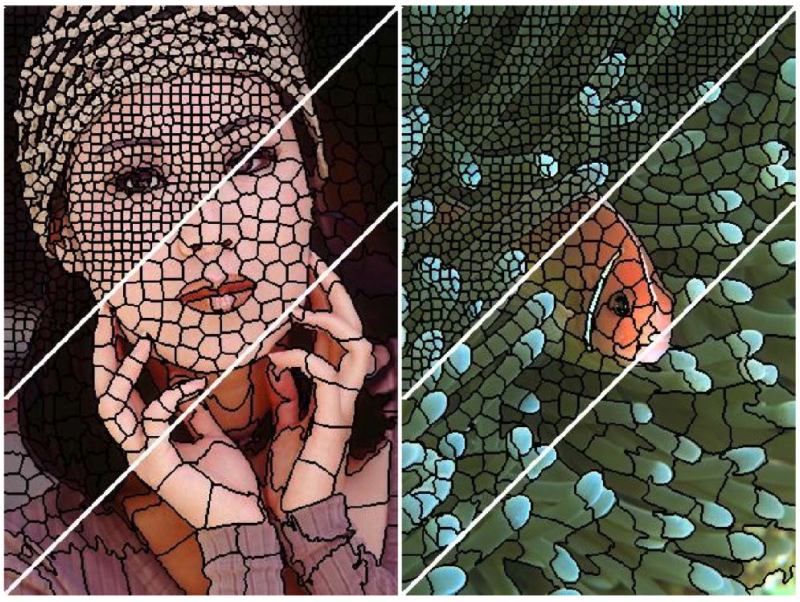
\includegraphics[scale=0.3]{fig/superpixels}
	\caption{Visualization of image segmentation using SLIC \citep{Achanta2012}}
	\label{fig:superpixels}
\end{figure}

When constructing superpixels, there are some properties of the algorithm that are desirable, regardless of the problem that are being solved. These are, according to \citep{Achanta2012}, the following three points:

\begin{itemize}
	\item Superpixels should adhere well to image boundaries
	\item When used to reduce computional complexity as a preprocessing step, superpixels should be fast to compute, memory efficient, and simple to use.
	\item When used for segmentation purposes, superpixels should both increase the speed and improve the quality of the results.
\end{itemize}

\cite{Achanta2012} proposes a superpixel-segmentation algorithm (SLIC), which in their opinion is best suited to meet these demands. They compare their algorithm to a variety of state-of-the-art superpixel methods, and conclude that none of the existing methods are satisfactory in regards to the points.

\subsubsection{Simple Linear Iterative Clustering (SLIC)}
The SLIC algorithm is fairly simple to understand. One of its key principles is that, by limiting the search space for each cluster center (points in the regular raster grid), it reduces the search speed significantly. This is achievable due to the fact that one of the primary goals of algorithm is to create a set of approximately equal sized superpixels. Thus, instead of searching the whole raster grid for each cluster center, the algorithm only has to search for edge pixels at a distance equal to D, as shown in \autoref{eq:distanceSuperpixel}.

\begin{equation}
	D'=\sqrt{\left(\frac{d_{c}}{m}\right)^{2} + \left(\frac{d_{s}}{S}\right)^{2}}
	\label{eq:distanceSuperpixel}
\end{equation}

In \autoref{eq:distanceSuperpixel} $d_{c}$ is the euclidean distance between two pixels in terms of color and $d_{s}$ is the pixels euclidean, spatial distance. Furthermore, $S$ is the sampling interval of the cluster centers ($S = \sqrt{N/k}$, where N is the number of pixels in the grid and k is the desired number of superpixels) and $m$ is a fixed constant based on the color diversity in the image.

Since the algorithm generates superpixels by clustering pixels based on their color and spatial proximity, creating a 5 dimensional, \textit{labxy} space, one would think that the distance could be found by simply taking the 5D euclidean distance. However, it turns out that for large superpixels, spatial distance outweigh the color proximity. Which is why the two distances $d_{c}$ and $d_{s}$ are weighted.

\subsection{Artificial Neural Networks for shape detection}
In recent years, the development of machine learning, a branch of artificial intelligent systems, has become increasingly important in terms of pattern and object recognition in remote sensing and image analysis in general. One of the most commonly used approaches for data mining in remote sensing, has been artificial neural networks \cite{Lary2016}.

The basic principle behind artificial neural networks (ANNs) is that it is built up by a network of many simple units that are working in parallel with no centralized control unit. The networks primary means of storage are the weights between the individual units, and the network learns by updating these weights in relation to being provided with a training example.

In order to understand the behavior of ANNs it is important to understand their structures. The most common structure for an ANN is what is called a Feed-forward neural network structure.

\subsubsection{Feed-forward neural networks}
A feed-forward neural network is build up by a given number of connected layers. A layer is a collection of simple units, called artificial neurons. All networks must consist of an input and output layer, but can also contain an optional number of hidden layers. A network that only consists of an input and output layer is called a perceptron, and it has been shown that these types of networks are only able to model linear functions \citep{Minsky1969}.

\paragraph{Input Layer}
The input layer is the layer that feeds the information into the network. Here the number of neurons are typically equal to the number of features in the data.

\paragraph{Hidden layer}
The hidden layers in an ANN is what enables the network to learn and model nonlinear functions. It is the weights on the connections between the different layers that enables the network to encode the information extracted from the training data.

\paragraph{Output layer}
In order to extract the answer or prediction from the model, an output layer has to be present. Depending on the setup of the neural network, the output value can either be a real value or a set of probabilities. The output type is dependent on the activation that is chosen for the layer. What an activation function is, and how it effects the output of a layer will be discussed later in this section.

A feed forward network can either be fully og partly connected. In a fully connected network, all the neurons in each layer has a connection to all neurons in the previous layer, and all neurons in the next layer, while in a partly connected layer only some of the neurons are connected.

\subsubsection{Training a neural network}
The main purpose of a well trained ANN is to be able, by using its weighted connections, to amplify the signal and dampen the noise of the data it has been trained on. It does so by altering the different weights and biases in a way that allocates significance to some features and removing it from other. This way the model can learn which features are tied to which outcomes.

Neural networks learn these relationships by making a guess based on the input, weights and biases, and then get feedback on how accurate the guess was. It is the loss function related to the model, such as stochastic gradient decent (SDG), which gives this feedback by rewarding good guesses and penalizing bad ones.

The most common learning algorithm associated with neural networks is the \textit{backpropagation learning algorithm}.

\subsubsection{Backpropagation learning}
The backpropagation algorithm learns by first trying to compute a training examples output value, by taking a forward pass through the network. If the output matches the label associated with the example nothing happens, but if it does not the weights has to be updated.

In order to update the weights in the network, \autoref{eq:backupdate} is used.

\begin{equation}\label{eq:backupdate}
	W_{j,i} \Leftarrow W_{j,i}+ \alpha*a_{j}*Err_{i}*g'(input\_sum_{i})
\end{equation}

\autoref{eq:backupdate} is called the weight update rule for the connection between neuron $j$ and $i$ as seen in \autoref{fig:backpropagationtwolayers}. Furthermore, $\alpha$ is the learning rate (discussed in \autoref{section:hyperparameters}), $a_{j}$ is the incoming activation function, $Err_{i}$ is the error in $i$ and $g'(input\_sum_{i})$ is the derivative of the activation function over the input sum as seen in \autoref{eq:activation}.

\begin{equation}\label{eq:activation}
a_{j} = g(input\_sum_{j})
\end{equation}

where the input sum is given by:

\begin{equation}\label{eq:inputsum}
	input\_sum_{i} = W_{i}*A_{i}+b
\end{equation}

\begin{figure}[!h]
	\centering
	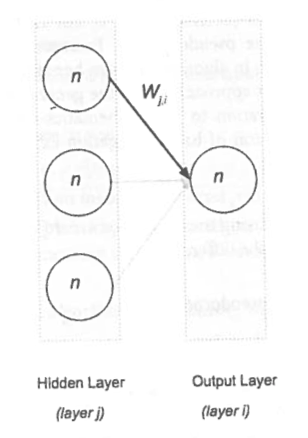
\includegraphics[scale=1]{fig/backpropagation_two_layers.png}
	\caption{The two last layers of an multilayer feed-forward neural network \cite{Patterson2017}}
	\label{fig:backpropagationtwolayers}
\end{figure}

The backpropagation algorithm traverses the network backwards, updating the weight of connection between each layer, as describd in \autoref{eq:backupdate}, until it reaches the input layer. This way the weights and biases that have been assigned the blame for the error are reduced, while the ones that supporting the correct answer are strengthened. 

\subsubsection{Activation functions}
Activation functions are scalar-to-scalar functions which are used to propagate the output of one layer to the next, and it is what enables the network to model nonlinear functions. This section will discuss some of the most common activation functions used in ANNs.

\paragraph{Linear}
The linear activation function, $f(x) = Wx$ is the simplest activation function and is often associated with the input layer of the network. It says that the dependent variable $x$ is proportional with the independent variable $Wx$.

\paragraph{Sigmoid}
The sigmoid activation function belongs to the class of logistic activation functions. It reduces extreme values or outliers in the example data, without removing them. One could see the sigmoid function as a machine that coverts independent variables of near infinite range into probabilities between 0 and 1.

\paragraph{Tanh (and Hard Tanh)}
Another class of activation functions are the hyperbolic trigonometric functions. The tanh function represents the ratio between the hyperbolic sine sine to the hyperbolic cosine, which means that unlike the sigmoid function, it has a normalized range between -1 and 1. The hard tanh activation function simply adds hard caps to the range, setting all values larger than 1 and smaller than -1 to respectively 1 and -1. The advantage of these functions are that they can deal more easily with negative numbers.

\paragraph{Softmax}
The softmax function, also referred to as the normalized, exponential function, is a generalization of the logistic function. Its function is that it returns the probability distribution over mutually exclusive output classes. For example, if the softmax activation function was applied to the vector [1, 2, 3, 4, 1, 2, 3], the result would be [0.024, 0.064, 0.175, 0.475, 0.024, 0.064, 0.175,]. As seen from this example, the function is most often used to weight the largest value and dampen values that are considerably smaller. 

\paragraph{ReLU}
The rectified linear unit function is currently considered the state of the art activation function. It can be described as $f(x)=max(0,x)$, meaning that it, above a certain threshold the output has a linear relationship with the dependent variable, it is else zero.

\subsubsection{Loss functions}
When working with artificial neural networks, we often talk about the ideal state of the network, meaning the state that classifies all the examples correctly. The loss function is a way of quantifying how close a network is to this ideal state. This is done by aggregating the errors produced by the networks prediction over the entire dataset, and average this value to get a single number that represents how close the network is to its ideal state. In other words, by minimizing the loss function, the network gets as close as possible to its ideal state, resulting in an optimization problem where the solution can be approximated well with iterative optimization algorithms.

There are different loss functions that are appropriate for regression and classification problems, however for the purpose of this project report it is only relevant to discuss the ones related to classification problems.

\paragraph{Hinge loss}
For hard classification, for example with discrete classes [sell=0, buy=1], the hinge loss function is most commonly used. It is also used by a class of models called maximum-margin classification models such as support vector machines, which are discussed in \autoref{section:svm}.

\paragraph{Logistic loss}
Often probabilities are of greater interest than hard classifications, in such situations the logistic loss function is of more value. An important remark when computing probabilities, is that all values has to be in the range 0 to 1 and that the probability of mutually exclusive outcomes should sum up to 1. Therefore, it is essential that the last layer uses the softmax activation function.

Optimizing the logistic loss function is the same as optimizing the "maximal likelihood", which means that the algorithm should maximize the probability that it predict the correct class, and do so for each single sample in the dataset. 

NOT FINISHED HERE

\subsubsection{Hyperparamenters}\label{section:hyperparameters}
In machine learning, hyperparameters deal with controlling the optimazation functions during learning, making sure that they neither overfit or underfit the data, but at the same time learns as quickly as possible.

\paragraph{Learning rate}
The learning rate, as seen in \autoref{eq:backupdate}, is a coefficient that scales the size of each weight update step. In other words, the learning rate decides how much of the computed gradient that should be used for each step. 

\paragraph{Regularization}
Regularization is important in order to control what is called out-of-control parameters. This is done by controlling the trade-off between finding a good fit on the training data and limiting the weight on features with high-polynomials. This is because such features tend to overfit the training examples.

\paragraph{Momentum}
Momentum is often described as the the learning rate of the learning rate. What it does is to prevent the learning algorithm from getting stuck in local minimas.

\paragraph{Sparsity}
Lastly, the sparsity hyperparameter helps recognize which features of the input examples that are relevant. This is important because in some datasets, the feature arrays for each example will be very different in terms of values.


\subsection{Support vector machines for shape recognition}\label{section:svm}
In machine learning, support vector machines (SVM) are supervised learning models used for classification and regression analysis. 

In a SVM model training examples are represented as points in a n-dimensional space, mapped so that the examples belonging to separate categories are clustered together. One or more hyperplanes are then fitted in order to separate the different classes from each other. New data is then mapped into that same space and classified based on which side of the hyperplane they are mapped. SVMs are often called large margin classifiers because their goal is to separate the classes by fitting the hyperplanes between them in a way so that the planes has the highest possible margin between the classes as shown in \autoref{fig:optimalmargin}.

\begin{figure}[!h]
	\centering
	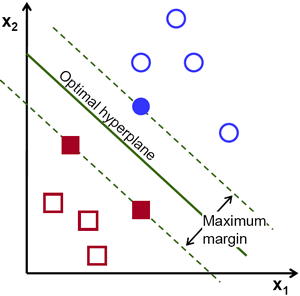
\includegraphics[scale=2.5]{fig/optimal-hyperplane.png}
	\caption{Example of optimal hyperplane for classification from \cite{Opencv2017}}
	\label{fig:optimalmargin}
\end{figure}

In order for support vector machines to work, the data points has to be separable by a plane. This is however not always possible in the dimension that the data is represented. In order to solve this issue SVM apply kernel functions.

Kernel functions enable SVM to operate in a high-dimensional, implicit feature space without ever computing the coordinates of the data in that dimension space. It simply computes the inner products between the images of all pairs of data in the feature space. This operation is often computationally cheaper than the explicit computation of the coordinates. In \autoref{fig:kernelfunction}  a 2-dimensional, non-separable dataset is mapped to a 3-dimensional, separable feature space.

\begin{figure}[!h]
	\centering
	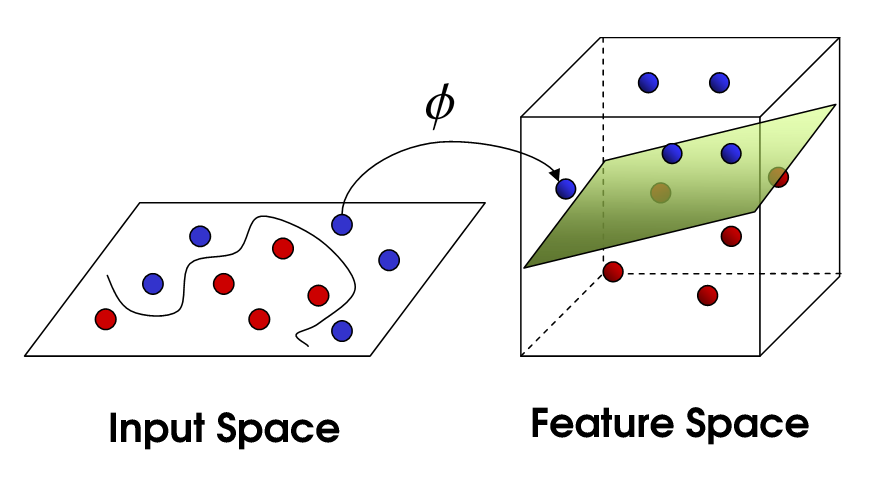
\includegraphics[scale=0.3]{fig/kernel_function.png}
	\caption{Classification using SVM with kernel function \cite{Opencv2017}}
	\label{fig:kernelfunction}
\end{figure}

\subsubsection*{Decision Trees}
Decision tree learning is one of the simplest and yet most successful forms of machine learning. They are learned top-down, and they use a recursive learning technique.

A decision tree represents a function that takes as input a vector of attribute values and returns a “decision” - a single output value. Furthermore, it is worth mentioning that decision trees are only good for some kind of functions.

Links:

https://www.pyimagesearch.com/2014/10/20/finding-shapes-images-using-python-opencv/\\
https://www.pyimagesearch.com/2016/02/08/opencv-shape-detection/
\\
http://melvincabatuan.github.io/SLIC-Superpixels/
\\
